\documentclass[xcolor=dvipsnames,table]{beamer}

\usepackage{latexsym}
\usepackage[utf8]{inputenc}
\usepackage[brazil]{babel}
\usepackage{amssymb}
\usepackage{amsmath}
\usepackage{stmaryrd}
\usepackage{fancybox}
\usepackage{datetime}
\usepackage[T1]{fontenc}
\usepackage{graphicx}
\usepackage{graphics}
\usepackage{url}
\usepackage{algorithmic}
\usepackage{algorithm}
\usepackage{acronym}
\usepackage{array}

\newtheorem{definicao}{Definio}
\newcommand{\tab}{\hspace*{2em}}

\mode<presentation>
{
  \definecolor{colortexto}{RGB}{0,0,0}
 
  \setbeamertemplate{background canvas}[vertical shading][ bottom=white!10,top=white!10]
  \setbeamercolor{normal text}{fg=colortexto} 

  \usetheme{Warsaw}
}

\title{Noções Básicas de Grafos} 

\author{
  Esdras Lins Bispo Jr. \\ \url{bispojr@ufg.br}
  } 
 \institute{
  Teoria de Grafos \\Bacharelado em Ciência da Computação}
\date{\textbf{03 de maio de 2015} }

\logo{
\includegraphics[width=1cm]{images/ufgJataiLogo.png}}

\begin{document}

	\begin{frame}
		\titlepage
	\end{frame}

	\AtBeginSection{
		\begin{frame}{Sumário}%[allowframebreaks]{Sumário}
    		\tableofcontents[currentsection]
    		%\tableofcontents[currentsection, hideothersubsections]
		\end{frame}
	}

	\begin{frame}{Plano de Aula}
		\tableofcontents
		%\tableofcontents[hideallsubsections]
	\end{frame}
    
    \section{Pensamento}
	\begin{frame}{Pensamento}
  		\begin{center}
    		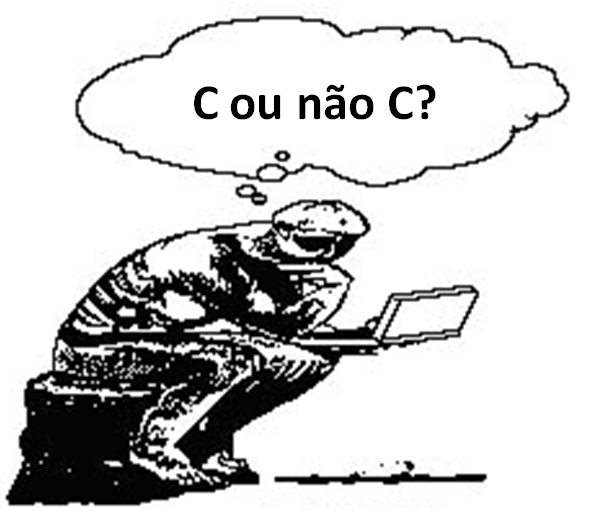
\includegraphics[width=7cm]{images/pensamento.png}
  		\end{center}
	\end{frame}
	
	\begin{frame}{Pensamento}
		\begin{columns}
			\column{.4\textwidth}  		
		  		\begin{center}
		    		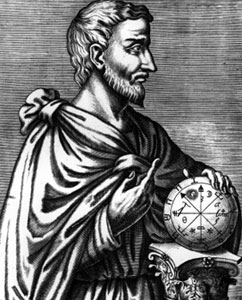
\includegraphics[width=.9\textwidth]{images/pitagoras.jpg}
		  		\end{center}
			\column{.6\textwidth}  		
				\begin{block}{Frase}
					\begin{center}
						{\large Em estado de dúvida, \\suspende o juízo.}
					\end{center}
				\end{block}		  		
		  		\begin{block}{Quem?}
		  			\begin{center}
						{\bf Pitagoras (571 a.C - 496 a.C)} \\Filósofo e matemático grego .
					\end{center}
				\end{block}
		\end{columns}
	\end{frame}
	
    \section{Sorteio para o Bônus}
    \begin{frame}{Bônus (0,5 pt)}
		\begin{block}{Desafio}
			\begin{itemize}
				\item Mostre que $\sqrt{2}$ é um irracional;
                \item Candidaturas até amanhã (03 de maio, 13h30);
                \item Apresentação e resposta por escrito $\rightarrow$ \\segunda (10 de maio, 15h30);
                \item 20 minutos de apresentação.
			\end{itemize}
		\end{block}
        \begin{block}{Sorteado}
			???
		\end{block}	
	\end{frame}
	
	\section{Noções Básicas de Grafos}	
	\subsection{Preliminares}
	\begin{frame}{Preliminares}
		\begin{block}{$V^{(2)}$}
			Para qualquer conjunto $V$, denotaremos por $V^{(2)}$ o conjunto de todos os pares não-ordenados de elementos distintos de $V$.
		\end{block}
		\pause
		\begin{block}{Corolário 1}
			Se $V$ tem $n$ elementos, então $V^{(2)}$ tem ${n \choose 2} := \frac{n(n-1)}{2}$ elementos.
		\end{block}
	\end{frame}
	
	\begin{frame}{Preliminares}
		\begin{block}{Corolário 2}
			Os elementos de $V^{(2)}$ serão identificados com os subconjuntos de $V$ que têm cardinalidade 2.
		\end{block}
		\pause
		\begin{block}{Corolário 3}
			Assim, cada elemento de $V^{(2)}$ terá a forma $\{ v,w \}$, sendo $v$ e $w$ dois elementos distintos de $V$.
		\end{block}
	\end{frame}
	
	
	\subsection{Grafo}
	\begin{frame}{Grafo}
		\begin{block}{Grafo}
			Um {\bf grafo} é um par $(V,A)$ em que $V$ é um conjunto arbitrário e $A$ é um subconjunto de $V^{(2)}$.
		\end{block}
		\pause
		\begin{block}{Vértices}
			São todos os elementos que pertencem a $V$.
		\end{block}
		\pause
		\begin{block}{Arestas}
			São todos os elementos que pertencem a $A$.
		\end{block}
	\end{frame}
	
	\subsection{Outras terminologias}
	\begin{frame}{Outras terminologias}
		\begin{block}{$\{v,w\} \equiv vw$}
			Uma aresta como $\{v,w\}$ será denotada simplesmente por $vw$ ou por $wv$.
		\end{block}
		\pause
		\begin{block}{Incidência}
			Diremos que a aresta $vw$ {\bf incide} em $v$ e em $w$. Também diremos que $v$ e $w$ são as {\bf pontas} da aresta.
		\end{block}
	\end{frame}
	
	\begin{frame}{Outras terminologias}
		\begin{block}{Ponta}
			Diremos que para uma aresta $vw$, $v$ e $w$ são as {\bf pontas} da aresta.
		\end{block}
		\pause
		\begin{block}{Adjacência}
			Se $vw$ é uma aresta, diremos que os vértices $v$ e $w$ são {\bf vizinhos} ou {\bf adjacentes}.
		\end{block}
		\pause
		\begin{block}{Observação}
			Nossa definição de grafo não admite que arestas tenham pontas coincidentes (i.e. laços). Existem autores que denotam este aspecto da definição dizendo que o grafo é ``simples''.
		\end{block}
	\end{frame}
	
	\begin{frame}{Outras terminologias}
		\begin{block}{$V(G)$ e $A(G)$}
			Se o nome de um grafo for $G$, então o conjunto de seus vértices será denotado por $V(G)$ e o conjunto de suas arestas por $A(G)$.
		\end{block}
		\pause
		\begin{block}{$n(G)$ e $m(G)$}
			O número de vértices de $G$ é denotado por $n(G)$ e o número de arestas por $m(G)$. 
		\end{block}
		\pause
		\begin{block}{Corolário}
			$n(G) = |V(G)|$ e $m(G) = |A(G)|$.
		\end{block}
	\end{frame}
	
	\begin{frame}{Outras terminologias}
		\begin{block}{$\overline{G}$}
			O complemento de um grafo $(V, A)$ é o grafo $(V, V^{(2)} \setminus A)$.
		\end{block}
		\pause
		\begin{block}{$K_n$} 
			O grafo $G$ é {\bf completo} se $A(G) = V(G)^{(2)}$. A expressão ``$G$ é um $K_n$'' é uma abreviatura de ``$G$ é um grafo completo com $n$ vértices''.
		\end{block}
		\pause
		\begin{block}{$\overline{K_n}$} 
			O grafo $G$ é {\bf vazio} se $A(G) =\emptyset$. A expressão ``$G$ é um $\overline{K_n}$'' é uma abreviatura de ``$G$ é um grafo vazio com $n$ vértices''.
		\end{block}
	\end{frame}
	
	\begin{frame}
		\titlepage
	\end{frame}
	
\end{document}